\newpage
\thispagestyle{empty}
\singlespacing
\chapter{Quantum walks with time-dependent Hamiltonians and their application to the search problem on graphs}
\onehalfspacing
The main goal of this thesis is to study quantum walks with time dependent Hamiltonians, focusing in particular on their application to the spatial search problem on graph. The general idea is trying to improve a time-independent implementation of quantum walks search using a time-dependent Hamiltonian analogous to the one used in the adiabatic evolution. In order to determine whether this new approach produces successfull results we study two selected graph topologies: the circular graph, for which the time-independent approach is not able to solve the search problem, and the complete graph for which the search problem is solved for both the time-independent and adiabatic evolution approaches. \\ We compare the two methods for the \textit{optimized-search}, \textit{localization} - which represents a search without needs to optimize the time - and a measure of \textit{robustness}.

\section{Search with time-dependent Hamiltonian}
In \Cref{sec:search quantum walk} we discussed the use of quantum walks for the spatial search problem \cite{Childs2004} and the application to the complete graph where the search problem is solved. We then illustrated how the adiabatic theorem can be used to solve computational problems with an adiabatic evolution of a quantum system \cite{Farhi2000}. Efforts to combine the two approaches showed that the search problem can be solved only with structures stronger than the usual Grover's oracle \cite{Wong2016}, thus making an \textit{Adiabatic-Quantum-Walk-Search} impossible. However this leaves space to a merely time-dependent quantum walk search, that takes advantage of a time-dependent implementation similar to the adiabatic evolution but that is not bounded to the strict adiabatic-theorem conditions and the limitation of the standard Grover's oracle.


    \subsection{Time-dependent quantum walks}
        Following from the adiabatic evolution discussed in the preliminaries, we consider a search Hamiltonian that interpolates between an initial Hamiltonian, i.e. the Laplacian of the graph $L$, and the final oracle Hamiltonian $H_w=\gamma\ket{w}\bra{w}$
          \begin{equation}
            H(s) = (1-s)L - s\gamma|w\rangle\langle w|
          \end{equation}
        where the interpolation schedule $s=s(t)$ goes from 0 to 1 as the time $t$ goes from 0 to the runtime $T$. \\ \\In order to find the evolved ground state of the beginning Hamiltonian we need to determine the evolution operator that for a time-dependent Hamiltonian is given by:
        \begin{equation}
          S(t,t_0) = \mbox{T } \mbox{exp}\Big\{ \frac{1}{i}\int_{t_0}^{t} dt' H(t')\Big\}
        \end{equation}
        where T is the time-ordering operator. Since we are only interested in the evolved state, having the exact evolution operator is somewhat irrelevant. \red{Additionally for the circular graph - which represents the main topology studied in this thesis - the search Hamiltonian does not show any particular properties making an analitical derivation of the operator not possible.} We therefore proceed by solving the differential Schroedinger equation:
        \begin{equation}
          i\frac{d}{dt}|\psi(t)\rangle = H |\psi(t)\rangle
        \end{equation}
        Recalling that we are dealing with matrices and vectors in an N-dimensional Hilbert space, we solve N-differential equations of the form
        \begin{equation}
        \frac{d}{dt}|\psi_i(t)\rangle = \sum_jH_{ij}|\psi_i(t)\rangle
        \end{equation}
        with the \red{boundary conditions $|\psi_i(0)\rangle = |\psi_i\rangle$.}\\

    \subsection{Interpolating schedule s(t)}\label{subsec:interpolating schedules}
        As pointed by Wong the interpolating schedule s(t) plays a crucial role in the evolution of the system and in the overall scaling of the algorithm.
        The original adiabatic evolution by Farhi and Gutmann \cite{Farhi2000} uses a linear interpolating schedule defined as $s_L(t) =\equiv \frac{t}{T}$. Roland and Cerf show that in order to obtain a quadratic speedup for the complete graph a non linear schedule is essential \cite{Roland2002}\cite{Morley2018}.

        Thus, from a linear interpolating schedule we consider also quadratic and cubic schedules:
        \begin{equation}
          s_S(t) \equiv \sqrt{\frac{t}{T}} \hspace{30pt} s_C(t) \equiv \sqrt[3]{\frac{t}{T}}
        \end{equation}
        We then consider the interpolating schedule analitically derived by Roland and Cerf for the unstructured search (complete graph) given by :
        \begin{equation}
            t = \frac{1}{2\epsilon}\frac{N}{\sqrt{N-1}}\Big[\mbox{arctan}\big(\sqrt{N-1}(2s-1)\big) + \mbox{arctan}\sqrt{N-1}\Big]
        \end{equation}
        By inverting the function, $s(t)$ is obtained as plotted in \cref{cerf}(a) \\
        As we have already mentioned in \Cref{subsec:local adiabatic} the shape of this interpolating schedule follows from gap $g(s)$ between the lowest two eigenvalues, changing faster when the gap is large, while it evolves slower when the gap is small. We therefore take these key aspects of $s(t)$ - derived for the unstructured search - and consider a similar interpolating schedule defined as follow
        \begin{equation}
            s_RC(t) = \frac{1}{2}(2(\frac{t}{T}-1)^{3}+1)
        \end{equation}
        \begin{figure}[ht]
          \centering
          \begin{tabular}{cc}
            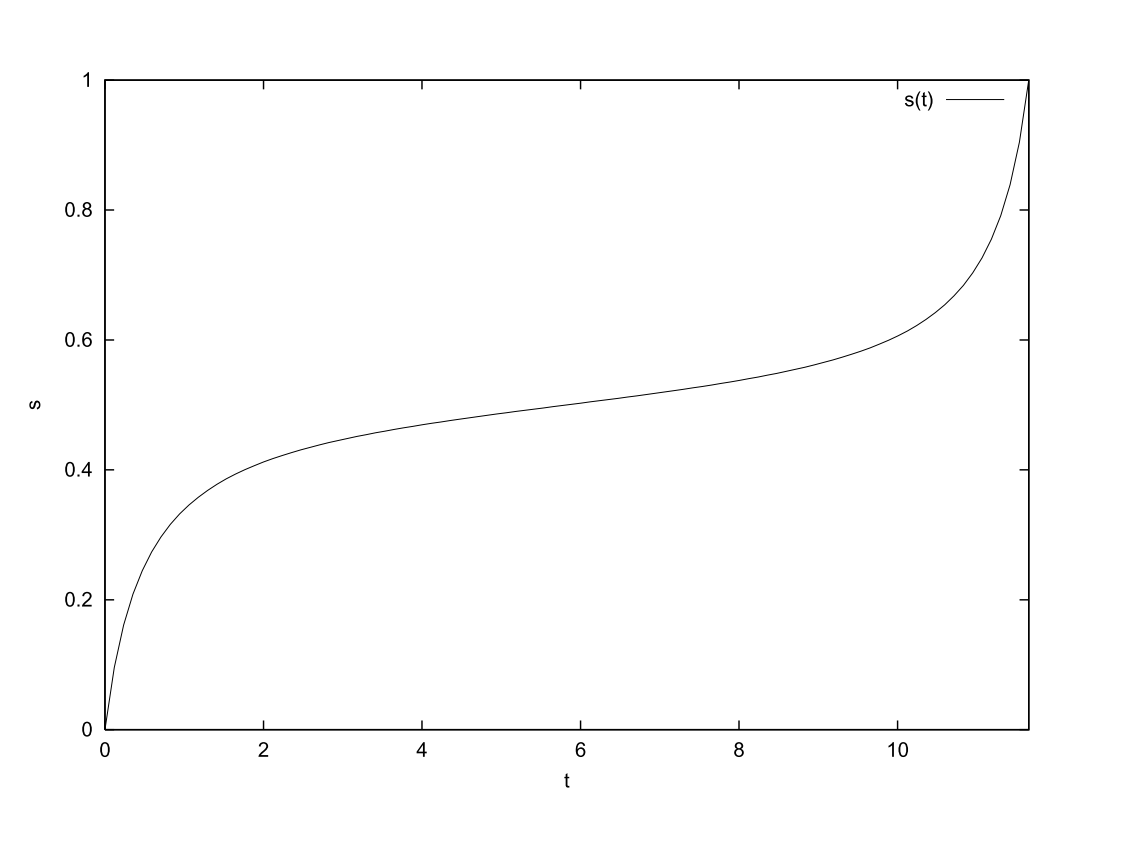
\includegraphics[width=75mm]{./figures/interpolating_schedules/cerf} &   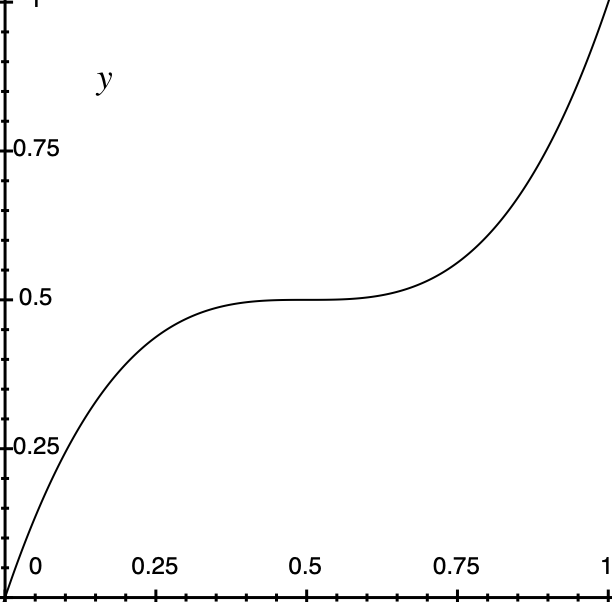
\includegraphics[width=45mm]{./figures/interpolating_schedules/our_cerf} \\
          (a) Original Roland-Cerf & (b) Roland-Cerf like\\[6pt]
          \end{tabular}
          \caption[Roland and Cerf's interpolating schedules for the unstructured search and our non-linear schedule]{\textbf{Roland and Cerf's interpolating schedule (a) and our Roland-Cerf like schedule (b).} These figures show the difference between the original interpolating schedule derived by Roland and Cerf for the unstructured search (left) and our Roland-Cerf like schedule(right). Although quite different we study the effects of this particular non-linear interpolating schedule and compare it with the linear one used by Farhi and Gutmann \cite{Farhi2000}.}
          \label{cerf}
        \end{figure}

        \subsection{Multiple runs for one search}\label{subsec:multiple_runs}
        To give a complete picture of the usefulness of the time-depedent approach, we consider the possibility of repeating the search multiple times. If the probability at which the solution is found is $p=1$ the search is \textit{perfect} and the problem is solved. However, if the proabability is less than one, i.e. \textit{imperfect search}, the problem can be solved by searching multiple times . Since the results of the search are checked independently, a single successfull search is sufficient, and this kind of routine is efficient as long as the probability $\big|\langle\psi(T)| w\rangle\big|^2$ is greater than $1/poly(N)$ (where N is the dimension of the graph) \cite{Morley2018} - which as we shall later see is verified for all the scenarios considered.

        Repeating the search multiple times does however come at a cost. It is indeed necessary to take into account for a non-zero \textit{initialization} time $t_{init}$ to prepare the system in the correct state as well a physical time for the measurement. Therefore, computing multiple searches with small $T$ becomes less efficient than less searches with larger $T$, where the quantity $t_{init}$ makes a lesser contribution to the overall $T$. Clearly this consideration is particularly relevant for increasing graph size.

\section{Selected topologies: circular and complete graph}
    Throughout our analysis we will focus on two selected graph topology, the cycle graph $Cy(N)$ and the complete graph $C(N)$. \\

    As previously discussed in \Cref{subsec:search qw complete graph, subsec:local adiabatic} the \textbf{complete graph} represents the best case scenario since it has been shown to solve the search problem both for the standard time-independent quantum walk approach \cite{Childs2004} and the local adiabatic evolution \cite{Roland2002}, with a quadratic speed up. An adiabatic implementation of the quantum walk search does not work with the usual Grover's oracle, requiring a more elaborate structure \cite{Wong2016}, however as we shall later see a merely time-dependent approach might give promising results in terms of robustness.  \\

    The \textbf{circular graph} on the other hand is not able to solve the search problem with the time-independent approach, and can give some interesting insights with the application of the time-dependent quantum walk search.  \\

    \red{Short statement needed to summarize the motivation for the selected topologies. Additionally it is necessary to decide whether to introduce the complete graph first thing or lastly.}

\section{Characterization of the results: Search, Localization and Robustness}
    Firstly it is necessary to define what type of results we are looking for. We begin by showing the difference between \textbf{search} and \textbf{localization}. Then we introduce a (not-so-rigorous) measure for the \textbf{robustness} of the search algorithm.

    \subsection{Search vs Localization}
      In order to study the performance of the search algorithms we have to characterize two particular classes of results, the (optimized)\textbf{search} and the \textbf{localization}, that help us decide whether the time-dependent approach brings any advantages.
      \begin{itemize}
          \item the (optimized) \textbf{search} describes the usual search, namely the finding of the solution with high probability (possibly unitary) for the smallest time as possible. As previously mentioned we also take into account the possibility of repeating the search multiple times.
          \item we call \textbf{localization} the finding of the solution with high probablity without the need to optimize the time. This description becomes necessary if we take into account the adiabatic nature of the time-dependent approach, that guarantees unitary probability for large $T$.
      \end{itemize}

    \subsection{Robustness}
        We've seen that the probability of a search problem depends on the time $T$ at which the quantum state is measured and the parameter $\gamma$. The optimal highest probability clearly is given by the optimal combination of $T$ and $\gamma$. These two parameters might be affected by noise or perturbation, leading to variation from the maximum probability. Therefore it is interesting to define a quantity that is able to quantify this fenomenon.

        Following from \cite{SH.HungS.Hietala2019} we define the \textbf{robustness},a quantitative measure representing the variation on the probability due to some perturbation/noise on $\gamma$.
        We begin by finding the highest probability $p$, evaluated with the single or multiple run for one search approach. For the corresponding $(T,\gamma)$ combination we evaluate the robustness as follows:
        \begin{equation}
            R ^\pm = p(T, \gamma) - p(T, \gamma \pm \delta)
        \end{equation}
        where $\delta$ is some positive perturbation of the $\gamma$ parameter. As we shall later see this quantity is given in terms of some percentage of $\gamma$. To find a unique value for the robustness an average of $R^\pm$ is done:
        \begin{equation}
            R = \bigg[\frac{R^++ R^-}{2}\bigg]^{-1}
            \label{eq:robustness}
        \end{equation}
        The quantity R should be positive\footnote{ Although not considered in our work, it is also possible to evaluate the robustness for non-maximal probability. In that particular scenario the value of the robustness could be negative.}, since the $(T,\gamma)$ combination corresponds to the hightest probability. Additionally we also notice that the perturbation on the parameter has equal probability of being positive or negative, thus the average ponderates between these two possibilities. \\

        \noindent
        As we mentioned, the variation in probability could also be due to some error on the time $T$ at which the state is measured. We can extend the measure of robustness to this particular scenario, where the value is similarly evaluated:
        \begin{equation}
            R ^\pm = p(T, \gamma) - p(T \pm \tilde{\delta}, \gamma )
        \end{equation}
        and $R$ follows directly from \Cref{eq:robustness}.
        In order to differentiate from this two measure of robustness we call them \textbf{$\bm{\gamma}$-robustness} and \textbf{$\bm{T}$-robustness} respectively.


        Although the value of $R$ does not have any absolute physical significance, it fits well for our specific scenario where the interest is focused on the comparison between two specific approaches. Therefore this quantity will be solely used to characterize a particular approach as \textbf{more} or \textbf{less robust}, where the first is characterized by having a larger value of robustness compared to the latter.

\section{Results for the Circular Graph}
We now address the results for the circular graph. We begin by evaluating the probabilities for the time-independent and the time-dependent Hamiltonians. We compare the localization of the two approaches, followed by the search - which requires the introduction of a new quantity that takes into account the possibility of doing multiple runs for one search. Lastly we study the robustness of the time-dependent approach and determine whether the newly introduced Hamiltonian makes the search more robust than the time-independent one.

    \subsection{Time-Independent Benchmarks}
        The first step of the analysis is to compute time-independent benchmarks. We computed the probability over a $(T,\gamma)$ grid, with $T\in[0,N]$ and $\gamma\in[0,2.5]$, where N is the dimension of the graph considered. An initial run of the probability distribution shows that the probability does not increase with time, thus the need to evaluate for $T$ greater than $T=N$ proved to be unnecessary. In addition, Grover's algorithm for the unstructured search has a time scaling of $O(\sqrt{N})$ and the Farhi and Gutmann's global adiabatic evolution is $O(N)$, thus focusing on $T \leq N$ suffices.\\
        \blue{2} \\
        Throughout the analysis we will consider graphs up to N = 71, with only odd dimensions which makes a easier oracle placement in the center vertex of the graph\footnote{The position of the oracle is somewhat irrelevant for the graph topologies considered, since every node is equivalent to all the $N-1$ others. Nevertheless odd dimensions allows to place the oracle in the central vertex of the graph, namely $\ket{\frac{N+1}{2}}$.}. Additional considerations and reasoning for the $(T,\gamma)$ grid can be found in the Appendix. \\


        To display the results in an intuitive way we used a heatmap plot, which gives a good idea on the probability distribution for varying combinations of $(T,\gamma)$: \\
        \blue{3}
          \begin{figure}[ht]
            \centering
            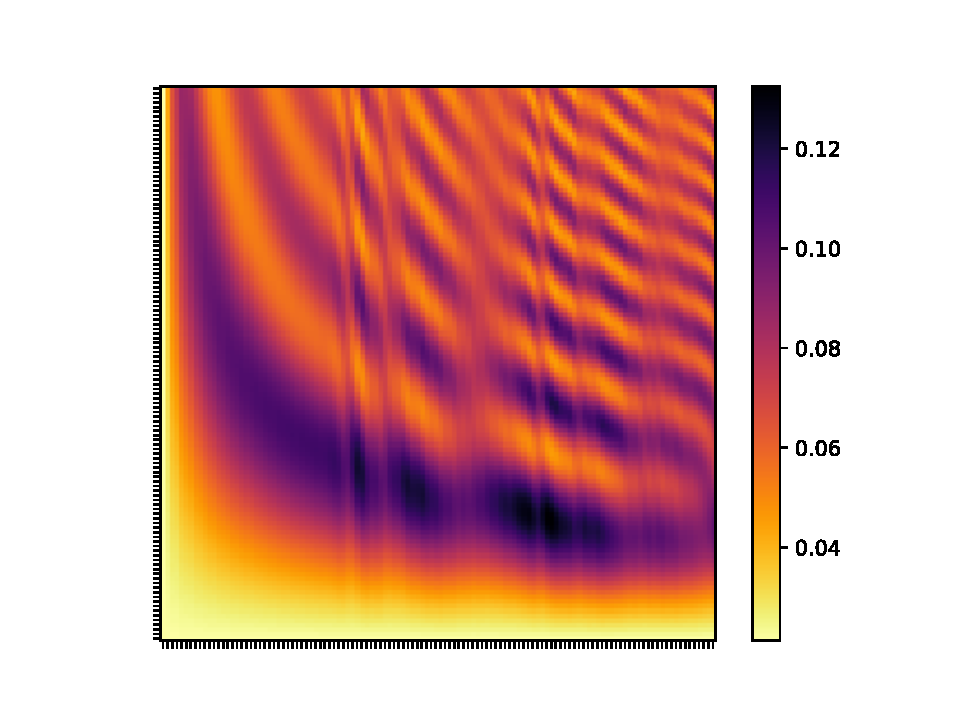
\includegraphics[width=9cm]{./figures/time_independent_benchmark_47}%
            \caption[Probability heatmap plot for the time-independent Hamiltonian, N=47]{\textbf{Probability heatmap plot for the time-independent Hamiltonian.} The figure shows the probability distribution for a circular graph of N=47 evaluated using the time-independent Hamiltonian, providing thus the necessary benchmark. Note that dark color do not represent probabilities close to one, but only higher probability regions.}
            \label{fig:heamap-independent}
          \end{figure}

        \subsubsection*{Comments on the probability distribution}
        From the heatmap plot we see that the probability distribution does not increase smoothly with increasing time, but shows peaks (dark regions) and valleys (lighter regions). Additionally high probability regions are scattered throughout the grid and do not appear necessarily for large $T$. We will later see that this is a weakness of the time-independent approach, since a small variation of the parameter $\gamma$ leads to possibly great variation of the probability.

    \subsection{Time-Dependent Results}\label{subsec:time_dependent_results}
        Similarly we compute the probability with the time-dependent Hamiltonian using the interpolating schedules introduced in \Cref{subsec:interpolating schedules}. To easily compare the two methods we consider the same time $T=N$ and $\gamma$ used for the time-independent benchmarks. Indeed, from an initial run we see that the $\gamma$ parameter affects the probability similarly to the time-independent approach, namely the probability tends to be higher for smaller values of $\gamma$. \\
        \blue{4}

        The probability is then evaluated for all the interpolating schedules $s(t)$ , and the results are again presented with an intuitive heatmap plot.
        \blue{5}

        \begin{figure}[ht]
        \centering
        \begin{tabular}{cc}
          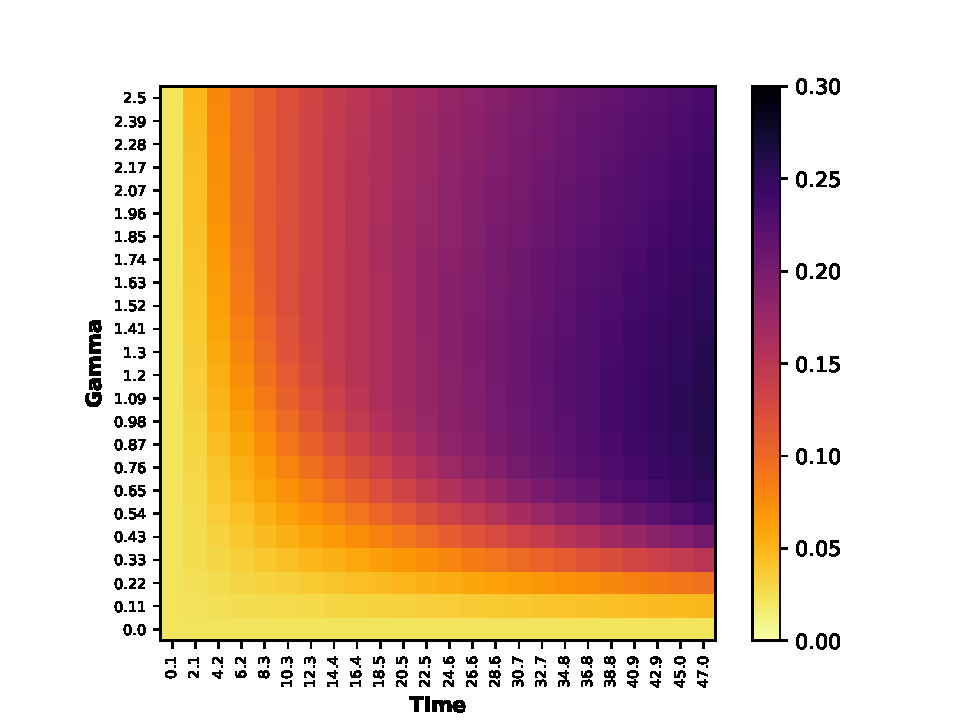
\includegraphics[width=75mm]{./figures/time_dependent_heatmap/47_heatmap_time_dependent_lin.pdf} &   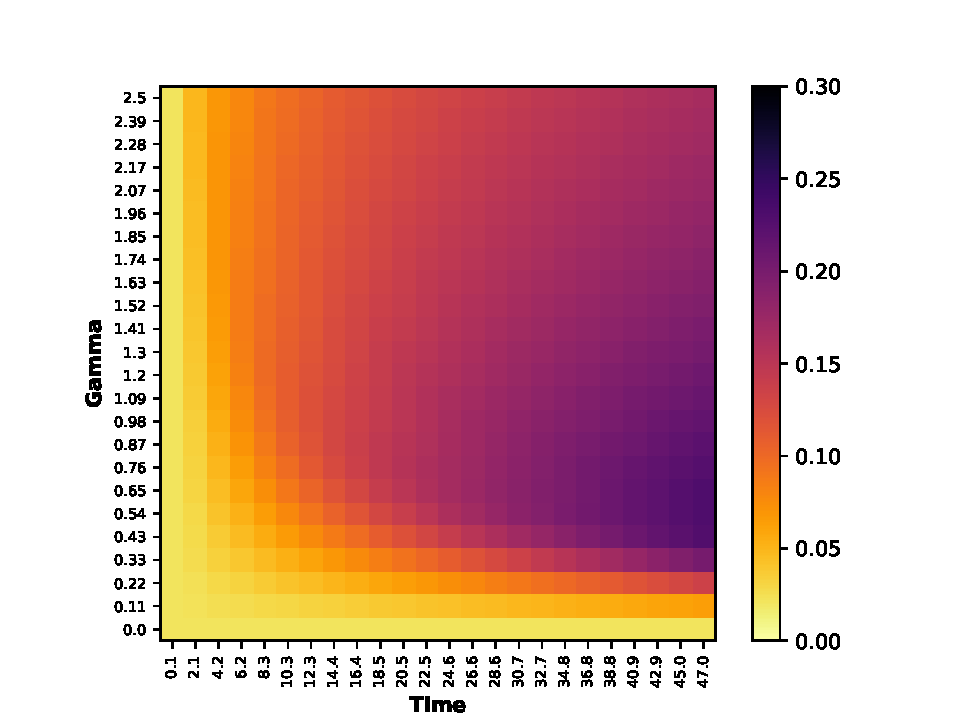
\includegraphics[width=75mm]{./figures/time_dependent_heatmap/47_heatmap_time_dependent_sqrt.pdf} \\
        (a) lin & (b) sqrt\\[6pt]
        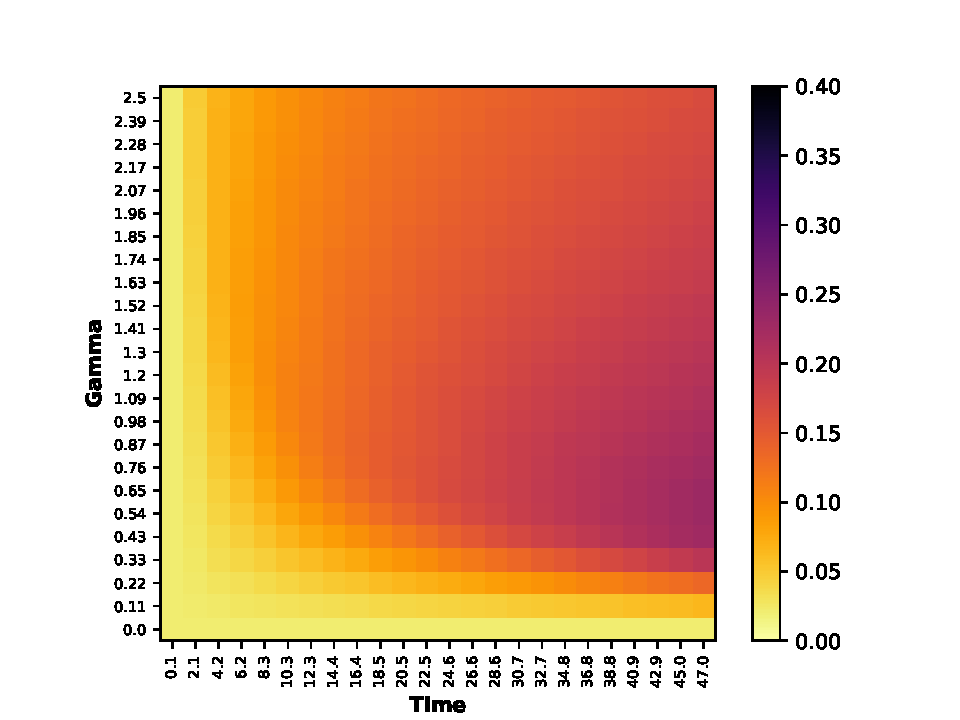
\includegraphics[width=75mm]{./figures/time_dependent_heatmap/47_heatmap_time_dependent_cbrt.pdf} &   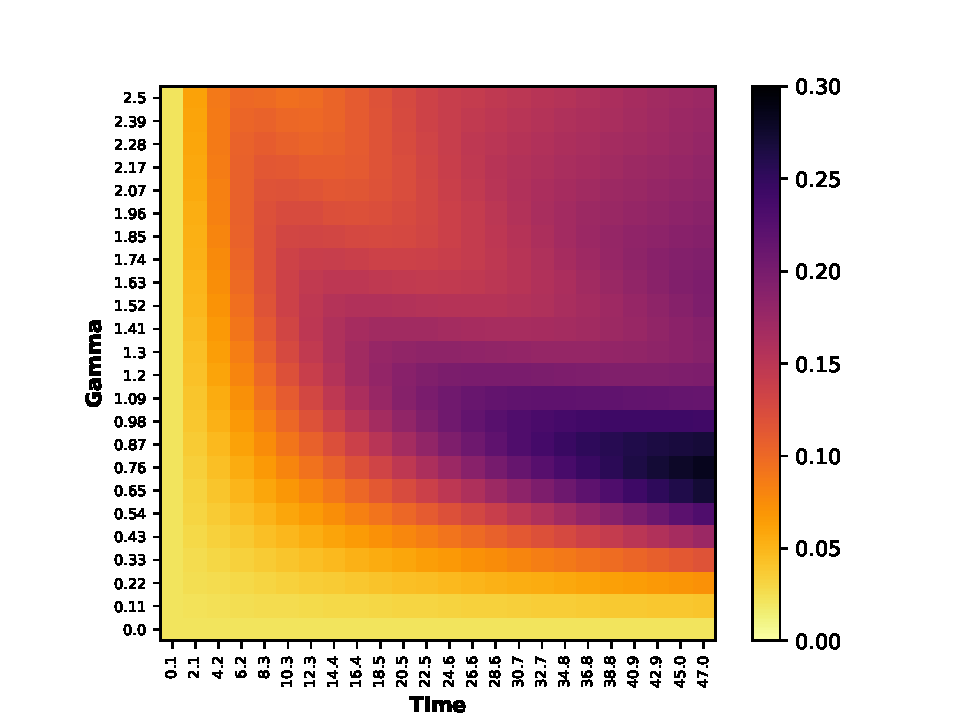
\includegraphics[width=75mm]{./figures/time_dependent_heatmap/47_heatmap_time_dependent_cerf.pdf} \\
        (c) cbrt & (d) cerf\\[6pt]
        \end{tabular}
        \caption[Probability heatmap plot for the time-dependent Hamiltonian, for different shapes of s(t)]{\textbf{Probability heatmap plot for the time-dependent Hamiltonian, for different shapes of s(t).} The figure shows the probability distribution for a circular graph of N=47 evaluated using the time-dependent Hamiltonian using the following interpolating schedules (a) linear, (b) $\sqrt{t/T}$, (c) $\sqrt[3]{t/T}$ and (d) Roland-Cerf(3). Note that the color gradient is normalized to p=0.3 to accentuate the difference in probability between different regions. }
        \label{fig:heatmap-dependent}
        \end{figure}
        \subsubsection*{Comments on the probability distribution}
        Compared to the time-independent hamiltonain approach we can clearly see that the probability distribution is smoother - has no valley and peaks - for both constant $\gamma$ and $T$ (any orizontal and vertical sections, respectively). In particular we notice that the probability increases for increasing time, and as we shall later see, for large enough $T$ it reaches probability equal to one.\\ If we look at the different interpolating schedules it is immediately evident that $s_S(t)$ and $s_C(t)$ schedules perform poorly compared to the linear $s_L(t)$. On the other hand $s_{RC}(t)$ schedule performs similarly to $s_L(t)$, but has a significantly different probability distribution  that might affect its robustness.

    \subsection{Comparison: Localization}\label{subsec:localization_results}
        We now compare the localization properties of the two algorithm. As we have already mentioned, from an intial look at the probability heatmap plots we discovered the following:
        \begin{itemize}
            \item \textbf{Time-Independent QW}: the time-independent based algorithm is not able to solve the search problem with a single iteration, making it necessary to run multiple searches. This implies that the approach does not show any localization properties, in fact the probability does not increase with time as seen in \Cref{fig:heamap-independent}.
            \item \textbf{Time-Dependent QW}: the time-dependent based search on the other hand solves the search problem with a single iteration, although that happens for large values of $T$, as can be seen in Figure?. This is indeed a consequence of the \textit{adiabatic inspired} implementation, for which at large $T$ the probability goes to one.
        \end{itemize}
        \blue{6}\\
        Although the time-dependent approach is able to get to unitary probability for large $T$, it is able to produce large enough probabilities in much less time, as we can see from this plot. This is a consequence of the fact that the probability does not grow linearly with time, thus needing larger $T$ closer it gets to $p=1$. \red{Spiegare meglio cosa vuol dire large enough}\\
        \blue{7}


    \subsection{Comparison: Search}
        In order to compare the two approaches for the search it is clear that we cannot simply consider the time at which the solution is found with unitary probability, since that particular $T$ does not exist for the time-independent approach and is not optimized for the time-dependent one as seen for the localization results. Therefore, as previously mentioned, we consider the possibility of doing multiple runs for one search. For this reason we introduce the following quantity
        \begin{equation}
          \tau = \min\bigg(\frac{T}{p}\bigg)_{T, \gamma}
        \end{equation}
        where the minimization is done over $T$ and $\gamma$ \footnote{Remember that the probability depends directly on the combination of $T$ and $\gamma$.}. The quantity $1/p$ represents the number of runs necessary to get to unitary probability (statistically), and combining it with $T$ gives the total time necessary get to $p=1$. Minimizing over the combination of $T$ and $p$ gives the smallest time necessary to solve the search problem with unitary probability using the multiple runs approach.\\ The minimization thus consists in finding for fixed $T$ the maximum probability, evaluating then the quantity $T/p$ and finding the minimum.


        \noindent
        Additionally, the number of runs performed - from now on referred to as \textbf{iterations} - given by
        \begin{equation}
          I = \min\big(p^{-1}\big)
        \end{equation}
        might give some useful insights on the performance of the approach, in particular if you take into account the initialization time $t_{init}$, since large number of $I$ are penalized by such $t_{init}$.\\


        \noindent
        However, this approach poses a few problems. In fact if we look at how the quantity $T/p$ varies for varying $T$, we discover that the minimum of such quantity will always be for the smallest $T$ available, regardless of the type of Hamiltonian and interpolating schedule $s(t)$ considered. The following plot indeed shows, for a sampled $\gamma$, the shape of $T/p$ with increasing time. \\
        \blue{8}
        \begin{figure}[ht]
        \centering
        \begin{tabular}{cc}
          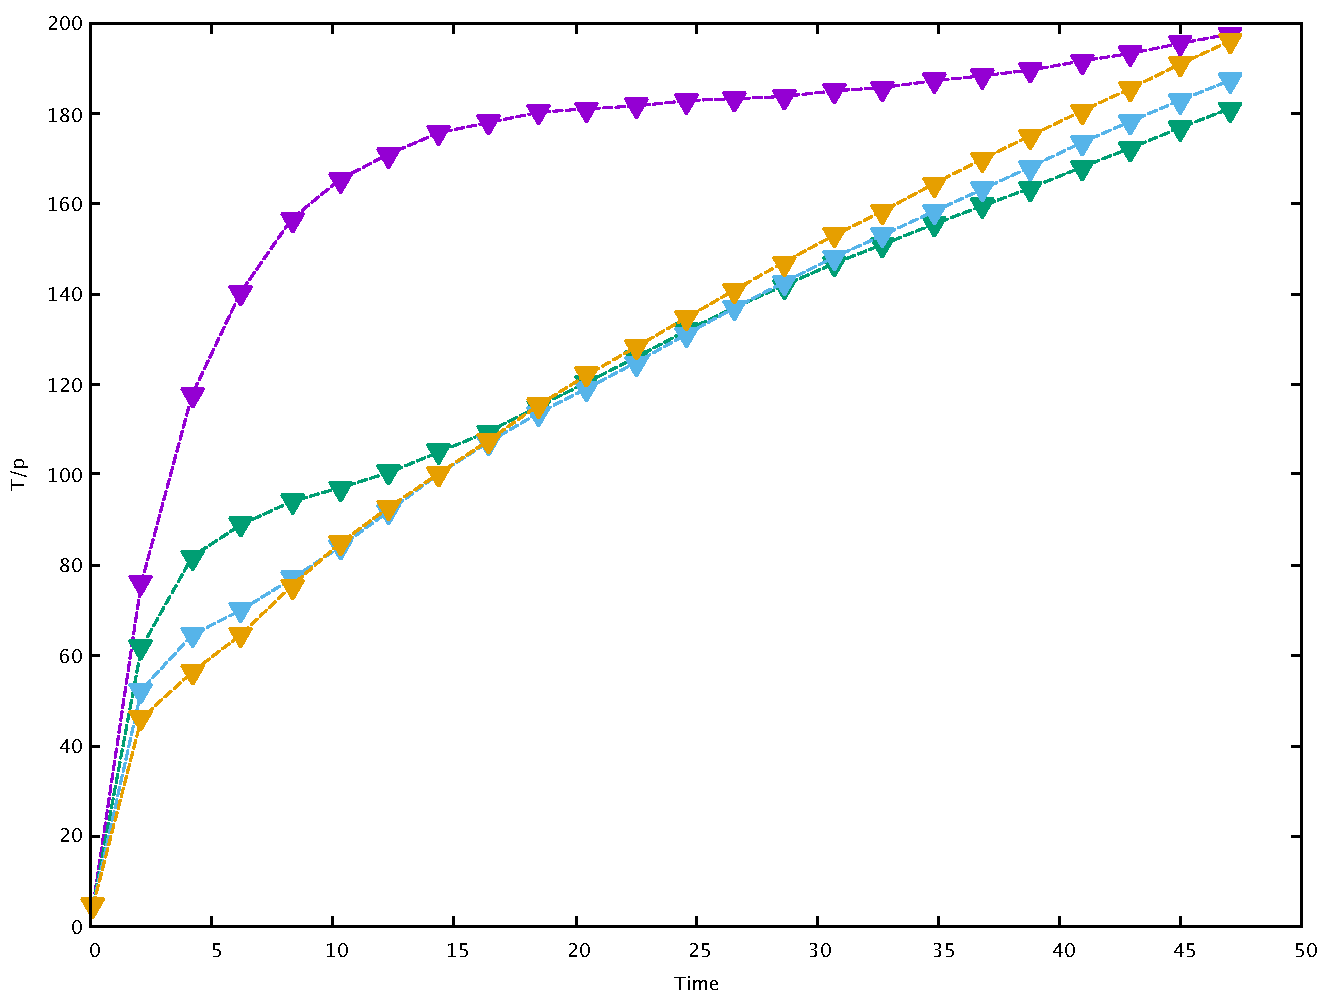
\includegraphics[width=75mm]{./figures/sampled_t_over_p/T_p_lin.pdf} &   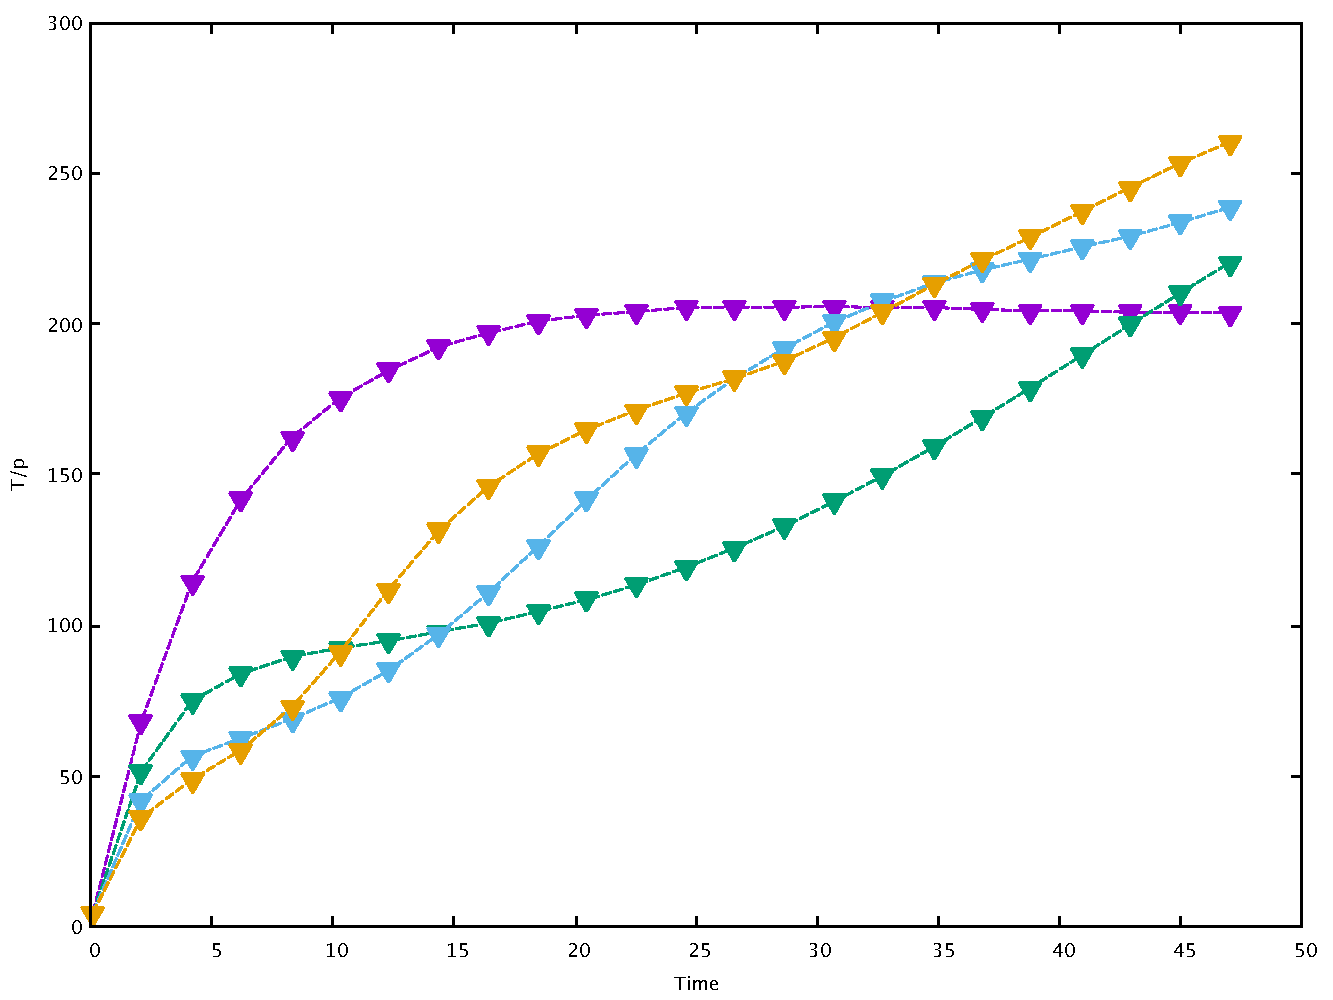
\includegraphics[width=75mm]{./figures/sampled_t_over_p/T_p_cerf.pdf} \\
        (a) lin & (b) Roland-Cerf\\[6pt]
        \end{tabular}
        \caption[$T/p$ distribution for sampled $\gamma$ showing that the minimum will always be for the smallest $t$ ]{\textbf{Distribution of the quantity T/p for sampled $\gamma$ showing that tthe min(T/p) will always be the smallest for the smallest $t$.}he figure shows the distribution of the quantity $T/p$ for some sampled values of the parameter $\gamma$, using the linear and Roland-Cerf interpolating schedules. It is clear that the quantity $\min(T/p)$ will always be for the smallest $T$ available, regardless of the interpolating schedule, requiring therfore a constrain on the time.}
        \end{figure}

        \noindent
        In addition, in \Cref{subsec:multiple_runs}  we mentioned that when dealing with multiple runs we need to take into account an initialization time $t_{init}$. It becomes therefore necessary to introduce a minimum value of time that can be considered, since for small $T$ the contribution given by $t_{init}$ can have a significant impact. We call this particular $T$ as \textbf{lower bound time}, reffered to as $T_{\min}$, and study its effect on $\tau$ and the overall performance of the time-independent and time-dependent algorithms. \\ \\

        \bpar{\bm{$\tau$} and $\bm{I}$ for increasing lower bound time \bm{\tmin}}
         We begin by studying how $\tau$ and $I$ vary with increasing lower bound time \tmin.
         In the following plot we show the shape of $T/p$ with the time-independent approach and the time-dependent one; since we're only interested in the general effect of \tmin on $\tau$ and $I$ we only consider the linear interpolating schedule $s_L(t)$\footnote{We have seen in \Cref{subsec:time_dependent_results} the probability distribution for the different interpolating schedules is quite similar, therefore looking only at $s_L(t)$ is sufficient.}. For sake of semplicity we study the cycle graph $Cy(51)$ with time up to $T=N$\\
         \blue{9}
         %TAU LOWER BOUND TIME
         %%%
%INTERPOLATING SCHEDULES: ORIGINAL ROLAND-CERF AND OUR S_RC
%%
\begin{figure}[ht]
  \centering
  \begin{tikzpicture}
    \begin{axis}[name=plot,
    xmin=0, xmax=60,
    ymin=0, ymax=600,
    width = 120mm,
    xlabel = Dimension $N$,
    ylabel = $\bm{\tau}$ ]
    \addplot[color=arancio,mark=*,mark size=2.5pt, x=a ,y=b] table{./Data/51_tau_lbt_static.txt};\addlegendentry{time-independent}
    \addplot[color=rossoscuro,mark=*,mark size=2.5pt, x=a,y=b] table{./Data/51_tau_lbt.txt};\addlegendentry{$s_L(t)$}

    \end{axis}
  \end{tikzpicture}
  \caption[$\tau$ distribution for increasing lower bound time.]{\textbf{\bm{$\tau$} distribution for increasing lower bound time. }The figure shows the $\tau$ distribution for increasing values of lower bound time, using the time-independent hamiltonian (orange) and time-dependent hamiltonain (red) and evaluated for a Cy(51). We see that for times smaller than a characteristic time $T^*$ the time-independent approach performs slightly better, while for large time the time-dependent one performs significantly better.}
  \label{fig:tau_increasing_time}
\end{figure}


        As we can see from the plot, the distributions can be divided into two sections marked by a particular $T^*$, representing the time at which the two distributions - time-dependendent and time-independent - intersect (for the time being the value of such time is not of our interest):
        \begin{itemize}
            \item for $T_{\min}<T^*$ the time-dependent approach has a comparable performance with the time-independent one, although the latter has a slight advantage.
            \item for $T_{\min}>T^*$ however the time-dependent approach performs significantly better, in particular with increasing \tmin
        \end{itemize}
        The behaviour for large T is to be expected, considering that the time-dependent approach shows localization properties and the probability increases with increasing time as we showed in \blue{7} and in \Cref{subsec:localization_results}, in contrast with the time-independent approach that does not show localization properties.\\ What this shows is that the choice of \tmin has a great impact on the outcome of our time-dependent approach, making it a successfull or unsuccesfull alternative. \red{manca qualcosa che dia una conclusione a quest'ultima affermazione}.\\

        \noindent
        Let's now look at the distribution of the number of iterations $I$. The following plots shows $I$ for increasing \tmin up to N, using the time-independent Hamiltonian and time-dependent one with the linear interpolating schedule $s_L(t)$.

        \blue{10}
        %PLOT ITERATIONS FOR LOWER BOUND TIME increasing
        %%%
%TIME INDEPENDENT: PROBABILITY FOR SAMPLED GAMMA
%%

%ITERS I DISTRIBUTION FOR INCREASING LOWER BOUND TIME

\begin{figure}[ht]
  \centering
  \begin{tikzpicture}
    \begin{semilogyaxis}[name=plot
    xmin=0, xmax=60,
    ymin=0, ymax=55,
    width = 120mm,
    xlabel = Dimension $N$,
    ylabel = $\bm{I}$ ]
    \addplot[color=verdescuro,mark=*,mark size=2.5pt, x=a ,y=b] table{./Data/51_iters_lbt_static.txt};\addlegendentry{time-independent}
    \addplot[color=bluscuro,mark=*,mark size=2.5pt, x=a,y=b] table{./Data/51_iters_lbt.txt};\addlegendentry{$s_L(t)$}

    \end{semilogyaxis}
  \end{tikzpicture}
  \caption[$I$ distribution for increasing lower bound time.]{\textbf{$\bm{I}$ distribution for increasing lower bound time. }The figure shows the distribution of $I$ for increasing values of lower bound time, using the time-independent hamiltonian (green) and time-dependent hamiltonain (blue) and evaluated for a Cy(51). This distribution reflects the probability distribution of the two approaches: for the time-independent hamiltonian the probability does not increase with time, resulting in a (almost) constant $I$, while the time-dependent hamiltonian showing localization properties requires less iterations to get to unitary probability.}
  \label{fig:iters_increasing_time}
\end{figure}


        The iterations distribution reflects the overall probability distribution of the time-dependent and time-independent Hamiltonian approaches. For small lower bound time the two approaches show a similar performance: the probability is very small, thus requiring a large number of iterations to get to unitary probability. As \tmin increases we see two very different trends:
        \begin{itemize}
            \item The time independent approach requires an almost constant number of iterations\footnote{The numerical value of $I$ is irrelevant since this distribution reflects only the Cy(51).}. This reflects the non-localization properties of this particular approach, for which the probability does not increase with time. It also shows that the maximum probability found is (almost) equal for all $T$, provided that \tmin is large enough.
            \item On the other hand the time-dependent approach requires less iterations to solve the search with unitary probability, as expected.
        \end{itemize}
        Taking into account that we are performing a multiple runs search and the initialization time $t_{init}$ previously discussed, it is clear that the time-depedent approch performs better than the time-independent counter part in most of the scenarios, where imposing a lower bound time \tmin becomes necessary.



        \bpar{\bm{$\tau$} and run iterations with constrained lower bound time}
        In order to show that the lower bound time does indeed have such a great impact on the performance of the time-dependent approach relative to the time-independent one, we study the distribution of $\tau$ and $I$ with a constrain on \tmin. It should be noted that in this particular scenario $\tau$ will no longer be a minimization over $T$ since the time is fixed, while the dependance on $\gamma$ remains. \\ \\ The choice of constrain is arbitrary and somewhat biased since the larger the constrain the better the performance of the time-dependent approach, as we've just shown in \blue{9}. Therefore, to make the choice fair, we consider the lower bound time to be $T_{\min} = \frac{\pi}{2}\sqrt{N}$ which is the same order of magnitude of the standard Grover's time scaling, the time-independent quantum walk search on the complete graph and the unstructured local adiabatic search. In the best-case scenario we might discover that the number of iterations necessary to get to unitary probability remains constant regardless of the dimension of the graph, making this approach have the same time scaling as the ones just mentioned; in the most probable scenario we discover that the number of iterations increases with the graph size, thus adding a scaling factor that depends on some power of N. \\

        \noindent
        We begin by investigating the effects of the interpolating schedule $s(t)$ on the $\tau$ distribution. The following plot shows the results for cycle graphs $Cy(N)$ with N up to 71, using the time-dependent hamiltonian and the interpolating schedules defined in \Cref{subsec:interpolating schedules}.\\
        \blue{11}

        As we could have expected the Roland-Cerf interpolating schedule $s_{RC}(t)$ performs the best, compared to the linear one. The $s_S(t)$ and $s_C(t)$ show poor performance compared to all the others, therefore are ignored for the next analysis.  This shows indeed that the shape of the interpolating function has a great impact on the performance of the algorithm, in particular when considering large graphs. We now compare the time-independent approach to the time-dependent one using the linear and Roland-Cerf interpolating schedules. Again, the time is constrained as in the previous plot. In particular we look at both the $\tau$ and $I$ distributions \\
        \blue{12}

        The following plot shows the number of iterations $I$ for the two considered approach. We are able to qualitatively describe the time scaling of the algorithms by superimposing the functions $\sqrt{N}$ and $\sqrt[3]{N}$: if the distribution of the iterations $I$ lies below the $\sqrt{N}$ line the time-dependent algorithm has some speedup compared to the classical search. Remember in fact that the overall time scaling of the multiple runs search is $\tau$, that is given by \\
        \blue{13}


    \subsection{Comparison: Robustness}
    We now address the robustness of the time-dependent and time-independent search. As we mentioned in Section? we are only interested in the comparison of the two approaches, and not an absolute measure of their robustness. Therefore we will use this measure solely as a comparison value. \\
    We proceed by considering small variations on the parameter $\gamma$ in the order of 1\% and 5\% (this numbers still need to be discussed). We begin by finding the quantity $\min(T/P)$ with time constrains ($T = 2\sqrt{N}$). For the corresponding $(T,\gamma)$ combination we evaluate the robustness R as defined in Section?
    For the time-dependent search with only consider the linear interpolating schedule an the Ronal-Cerf(3). As we showed in the previous section the Roland-Cerf Hamiltonian performs better than the linear conterpart, while from a qualitative point of view the linear Hamiltonian has a smoother probability distribution (see \cref{time_dependent_heatmap}(a)-(d)). The following plots show the semi-quantitative robustness for the $\gamma$ variations in the order of 1\% - 5\% for the time-independent search and the time-dependent one with linear and Roland-Cerf interpolating schedules s(t). \textbf{Computations are still needed}

    %ROBUSTNESS PLOT
    %%%
%PROBABILITY DISTRIBUTION FOR SAMPLED N, UP TO P=1
%%

\begin{figure}[ht]
\centering
  \begin{tikzpicture}
    \begin{axis}[name=plot
    xmin=0, xmax=441,
    ymin=0, ymax=1,
    width = 120mm,
    height=95mm,
    xlabel = $\bm{T}$,
    ylabel = $\bm{p}$,
    legend style={at={(0.95,0.05)},
    anchor=south east}]
    \addplot[color=verdescuro,no marks, thick, x=a, y=b] table{./Data/fig6/fig6_21_lin.txt};\addlegendentry{$N=21$, $\gamma=1.5$, $s_L(t)$}
    \addplot[color=verdescuro,dashed, no marks, thick, x=a, y=b] table{./Data/fig6/fig6_21_cerf.txt};\addlegendentry{$N=21$, $\gamma=1.05$, $s_{RC}(t)$}

    \end{axis}
  \end{tikzpicture}
  \caption{\textbf{Probability distibution for a $\bm{Cy(21)}$ with sampled $\bm{\gamma}$}: The figure shows the probability distribution for the cycle graph $Cy(21)$, evaluated with the time-dependent hamiltonian using the interpolating schedules (solid) linear $s_L$ and (dashed) Roland-Cerf $S_{RC}$. We can see that the probability increases with time, as expected. }
  \label{fig:probability_sampled_gamma}
\end{figure}



\section{Results for the Complete Graph}
    \subsection{Search results from Wong(2016)}
    \subsection{Localization results}
